
\فصل{نکات پیاده‌سازی}

\قسمت{یکپارچه‌سازی با \لر{Shell}}

در این قسمت ما با استفاده از کتابخانه \لر{ShellCEntryLib} تابع ورودی کد را مانند یک تابع ورودی عادی در \لر{C} کردیم. سپس با استفاده از دستور \لر{alias} در شل آن را مانند دستورات عادی کردیم. این کار دائمی است و بین دو بوت متوالی از بین نمی‌رود. همچنین با صدا زدن کد مانند \لر{memtest testname} می‌توان فقط یک تست خاص را اجرا کرد که در \رجوع{fig:impl1} قابل مشاهده است.

\قسمت{پیاده‌سازی چندهسته‌ای آزمون \لر{Identity}}

برای این کار ما از پروتکل \لر{MpService} در \لر{UEFI} استفاده کردیم. یک تابع کارگر ساختیم و سپس با استفاده از \لر{StartupAllAPs} آن را روی هسته‌های مختلف فراخوانی کردیم.

\begin{figure}
	\centering
	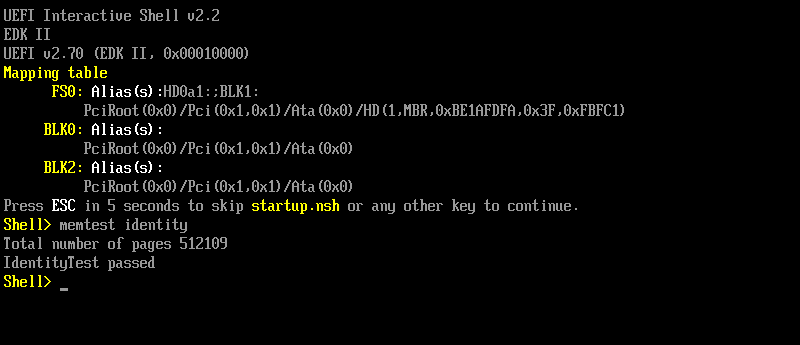
\includegraphics[width=0.7\linewidth]{figs/impl/impl1}
	\caption{صدا زدن برنامه و اجرای تست \لر{Identity}}
	\label{fig:impl1}
\end{figure}
